\section{Homotopy, star-shaped regions}
As homology is a functor $H_\ast:\mathbf{Top}\to\mathbf{Ab}$, it preserves isomorphisms: homeomorphic spaces have isomorphic homology. However, homology is not always able to distinguish between non-homeomorphic spaces. We introduce the looser notion of homotopy, which is a central concept of algebraic topology, and later we will show that homology is a homotopy invariant.
\begin{definition}
Let $f_0,f_1:X\to Y$ be two maps. A \emph{homotopy} from $f_0$ to $f_1$ is a map $h:X\times I\to Y$ such that $h(x,0)=f_0(x)$ and $f(x,1)=f_1(x)$. We say that $f_0$ and $f_1$ are \emph{homotopic} and write $f_0\sim f_1$.  This notation is justified because it is indeed an equivalence relation (transitivity follows from the gluing lemma).
\end{definition}
\begin{figure}
	\centering
	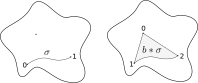
\includegraphics[width=0.5\linewidth]{assets/L05/05-homotopy}
	\caption{A homotopy $h$ between $f_0,f_1:X\to Y$.}
	\label{fig:05-homotopy}
\end{figure}

We denote by $[X,Y]$ the set $\mathbf{Top}(X,Y)/\sim$.

Suppose we have a map $g: Y\to Z$ and homotopic maps $f_0,f_1:X\to Y$, with a homotopy $h:f_0\sim f_1$. Then $g\circ h$ gives a homotopy $g\circ f_0 \sim g\circ f_1$. Similarly, if $g:W\to X$ is a map and $f_0,f_1:X\to Y$ are homotopic, then $f_0\circ g\sim f_1\circ g$.

If $g_0\sim g_1:Y\to Z$ and $f_0\sim f_1: X\to Y$, then $g_0\circ f_0\sim g_0 \circ f_1\sim g_1 \circ f_1$. Hence we are able to compose homotopy classes, giving the dotted arrow below.
\begin{equation*}
\xymatrix{\mathbf{Top}(Y,Z)\times\mathbf{Top}(X,Y)\ar[d]\ar[r] & \mathbf{Top}(X,Z)\ar[d]\\
[Y,Z]\times[X,Y]\ar@{-->}[r] & [X,Z]}
\end{equation*}

\begin{definition}
The \emph{homotopy category of topological spaces} is $\mathrm{Ho}(\mathbf{Top})$ whose objects are topological spaces and $\mathrm{Ho}(\mathbf{Top})(X,Y)=[X,Y]=\mathbf{Top}(X,Y)/\sim$.
\end{definition}
\begin{definition}
	A map $f:X\to Y$ is a \emph{homotopy equivalence} if $[f]\in[X,Y]$ is an isomorphism in $\htop$. In other words, there is $g:Y\to X$ such that $fg\sim 1_Y$ and $gf\sim 1_X$.
\end{definition}
This is an interesting category because it has \textit{terrible} categorical properties\todo{This sentence seems a bit random atm; give examples of why it's terrible? or just remove?}.

In Section \ref{lec:6-homotopy-invariance-of-homology} we will prove:
\begin{theorem}[Homotopy invariance of homology]
	If $f_0\sim f_1$, then $ H_\ast(f_0)= H_\ast(f_1)$.
\end{theorem}
This theorem states that the homology functor $H_\ast:\mathbf{Top}\to\mathbf{Ab}$ factors as $\mathbf{Top}\to\mathrm{Ho}(\mathbf{Top})\to\mathbf{Ab}$. In particular, it cannot distinguish between homotopy equivalent spaces. (Caution: spaces with isomorphic homology need not be homotopy equivalent.)
\begin{example}\label{exa:homotopy-equivalence-sphere}
The inclusion $S^{n-1}\subseteq \mathbf{R}^n-\{0\}$ is a homotopy equivalence. The homotopy inverse $p:\mathbf{R}^n-\{0\}\to S^{n-1}$ can be obtained by dividing a (always nonzero!) vector by its length. Clearly $p\circ i=1_{S^{n-1}}$. A homotopy $i\circ p\sim 1_{\mathbf{R}^n-\{0\}}$ is given by $(v,t)\mapsto tv+(1-t)\frac{v}{||v||}$. This example shows that homotopy equivalence does not preserve compactness.
\end{example}
\begin{definition}
A space $X$ is \emph{contractible} if the map $X\to\ast$ is a homotopy equivalence.
\end{definition}

\begin{definition}
	A \emph{star-shaped region} is a subspace $X$ of Euclidean space containing $\{0\}$, such that for all $x\in X$ and $t\in[0,1]$, $tx\in X$. 
\end{definition}
\begin{figure}
	\centering
	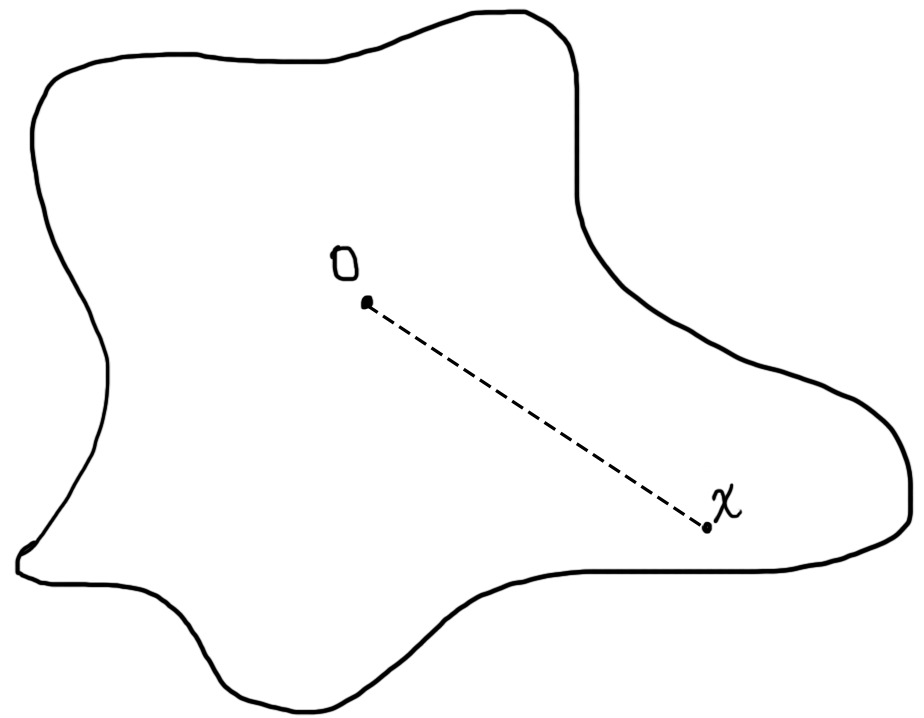
\includegraphics[width=0.4\linewidth]{assets/L05/05-star-shaped-region}
	\caption{A star-shaped region.}
	\label{fig:05-star-shaped-region}
\end{figure}

For example, any convex region containing the origin is star-shaped. An argument similar to the one in Example \ref{exa:homotopy-equivalence-sphere} shows that the inclusion of $\{0\}$ into a star-shaped region is a homotopy equivalence. Thus star-shaped regions are contractible. Our goal now is to prove the following.
\begin{theorem}\label{thm:star-shaped-homology}
	Let $X$ be a star-shaped region. The augmentation map $\epsilon: H_\ast(X)\to \mathbf{Z}$ is an isomorphism, i.e., $ H_0(X)\cong\mathbf{Z}$ and $ H_i(X)\cong 0$ for $i>0$.
\end{theorem}
%The strategy of proof is that $\epsilon$ is induced by sending $X\to \ast$. We'll look at the chain map $S_\ast(x)\to\mathbf{Z}\to S_\ast(X)$. We'll show that this composite induces the same map in homology as the identity map, which means that the identity map factors through $\mathbf{Z}$, so we're done. (probably not necessary to include this now that it's been moved to this section, given that the proof follows shortly)
Before proving this, we will give a notion of homotopy in the category of chain complexes.
\begin{definition}
Let $C_\bullet,D_\bullet$ be chain complexes, and $f_0,f_1:C_\bullet\to D_\bullet$ be chain maps. A \emph{chain homotopy} $h:f_0\sim f_1$ is a collection of homomorphisms $h:C_n\to D_{n+1}$ such that $\partial h+h\partial=f_1-f_0$.
\end{definition}
			\begin{equation*}
			\xymatrix{C_{n+2}\ar[r]^{f_1-f_0}\ar[d]^\partial & D_{n+2}\ar[d]^\partial\\
			C_{n+1}\ar@{-->}[ur]^h\ar[r]^{f_1-f_0}\ar[d]^\partial & D_{n+2}\ar[d]^\partial\\
			C_n\ar@{-->}[ur]^h\ar[r]_{f_1-f_0} & D_n}
			\end{equation*}
The following lemma shows the significance of this condition.
\begin{lemma}
	If $f_0,f_1:C_\bullet\to D_\bullet$ are chain homotopic, then $f_{0,\ast}=f_{1,\ast}: H(C)\to H(D)$.
\end{lemma}
\begin{proof}
	We show that $(f_1-f_0)_\ast=0$. Let $c\in Z_n(C_\bullet)(C)$, so that $\partial c=0$. Then $(f_1-f_0)_\ast c=(\partial h+h\partial)c=\partial hc+h\partial c=\partial hc$ is a boundary, which is zero in homology.
\end{proof}
\begin{proof}[Proof of Theorem \ref{thm:star-shaped-homology}]
	The maps $\{0\}\to X$ and $X\to \{0\}$ induce $\mathbf{Z}\xrightarrow{\eta}S_\ast(X)$ and $S_\ast(X)\xrightarrow{\epsilon}\mathbf{Z}$ respectively. It is clear that $\epsilon\eta = 1:\mathbf{Z}\to\mathbf{Z}$. We now proceed to show that $\eta\epsilon\sim 1:S_\ast(X)\to S_\ast(X)$. Note that the composite $\eta \epsilon$ kills all chains in dimensions greater than zero, and on zero-chains we have $\eta\epsilon(\sum a_ix_i)=(\sum a_i)c_0$ where $c_0$ is the zero-simplex at the origin.
	
\begin{figure}[H]
	\centering
	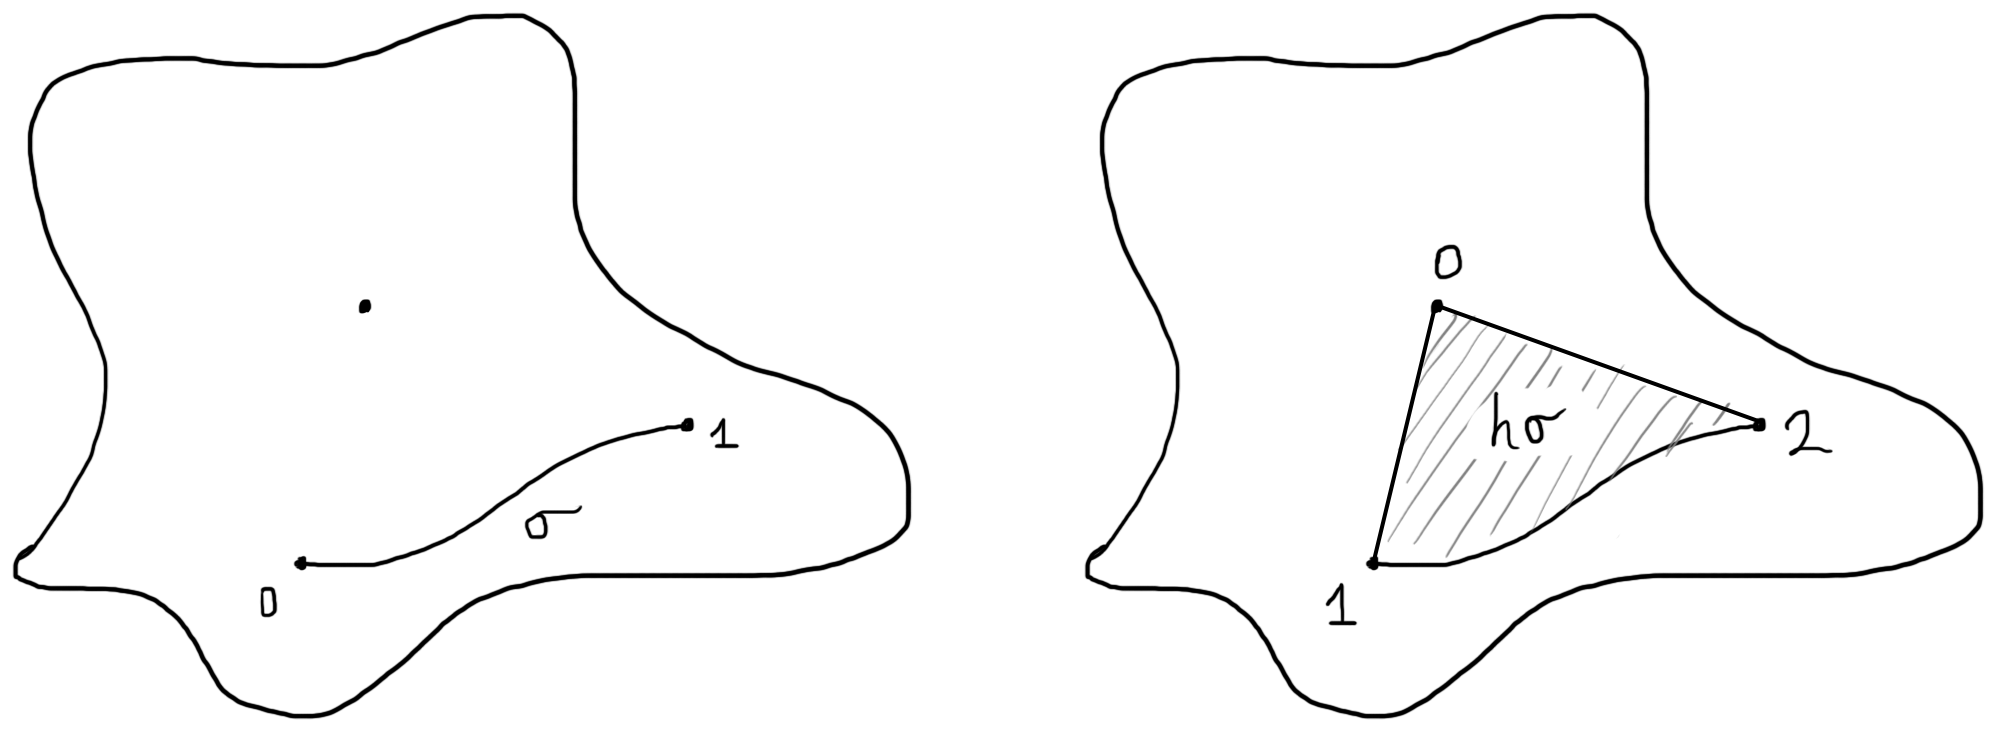
\includegraphics[width=0.8\linewidth]{assets/L05/05-star-shaped-line-homotopy-pf}
	\caption{The map $h$ illustrated on a 1-simplex.}
	\label{fig:05-star-shaped-line-homotopy-pf}
\end{figure}
	
	For $\sigma\in\Sin_q(X)$, define $h:\Sin_q(X)\to\Sin_{q+1}(X)$ as follows:
	$$h\sigma(t_0,\cdots,t_{q+1})=(1-t_0)\sigma\left(\frac{(t_0,\cdots,t_{q+1})}{1-t_0}\right).$$
	This extends by linearity to a map $h:S_q(X)\to S_{q+1}(X)$.
	Observe that $d_0 h \sigma = \sigma$, and if $q \geq 1$, $d_i h \sigma = h d_{i-1} \sigma$. Then, if $\sigma \in \Sin_q(X)$ with $q \geq 1$,
	\begin{align*}
		\partial h \sigma &= \sum_{i=0}^{q+1} (-1)^{i} d_i h\sigma\\
		&= \sigma - h \sum_{i=0}^q (-1)^i d_i \sigma\\
		&= \sigma - h\partial \sigma\\
		\partial h \sigma + h \partial \sigma &= \sigma.
	\end{align*}
	If $\sigma \in \Sin_0(X)$, then $d_1 h \sigma = c_0$ and we instead get $\partial h \sigma + h \partial \sigma = \sigma - c_0$. Thus $h:S_q(X)\to S_{q+1}(X)$ is a chain homotopy $\eta \epsilon \sim 1$ as desired.
\end{proof}
% Continue indenting like this.
